%%%%%%%%%%%%%%%%%%%%%%%%%%%%%%%%%%%%%%%%%
% FRI Data Science_report LaTeX Template
% Version 1.0 (28/1/2020)
% 
% Jure Demšar (jure.demsar@fri.uni-lj.si)
%
% Based on MicromouseSymp article template by:
% Mathias Legrand (legrand.mathias@gmail.com) 
% With extensive modifications by:
% Antonio Valente (antonio.luis.valente@gmail.com)
%
% License:
% CC BY-NC-SA 3.0 (http://creativecommons.org/licenses/by-nc-sa/3.0/)
%
%%%%%%%%%%%%%%%%%%%%%%%%%%%%%%%%%%%%%%%%%


%----------------------------------------------------------------------------------------
%	PACKAGES AND OTHER DOCUMENT CONFIGURATIONS
%----------------------------------------------------------------------------------------
\documentclass[fleqn,moreauthors,10pt]{ds_report}
\usepackage[english]{babel}
\usepackage{textcomp}
\graphicspath{{fig/}}




%----------------------------------------------------------------------------------------
%	ARTICLE INFORMATION
%----------------------------------------------------------------------------------------

\usepackage{adjustbox}

% Header
\JournalInfo{FRI Natural language processing course 2024}

% Interim or final report
\Archive{Project report} 
%\Archive{Final report} 

% Article title
\PaperTitle{Qualitative Research on Discussions - text categorization} 

% Authors (student competitors) and their info
\Authors{Ana Petrova, Žan Korošak and Bojan Ilić}

% Advisors
\affiliation{\textit{Advisors: Slavko Žitnik}}

% Keywords
\Keywords{discourse analysis, text categorization, language model}
\newcommand{\keywordname}{Keywords}


%----------------------------------------------------------------------------------------
%	ABSTRACT
%----------------------------------------------------------------------------------------

\Abstract{
Text categorization of online discussions involves classifying user-generated content into predefined categories to enhance understanding and analysis. This project focuses on a dataset sourced from an online discussion about "The Lady, or the Tiger?". Each entry is labeled according to discussion type, such as Seminar, Deliberation, Social, and others. We employed several different AI models and approaches for text classification and conducted an in-depth analysis of incorrect predictions to understand the challenges that this task presents. First we take a look at traditional approaches to text classification, such as Multinomial Naive Bayes, Random forest, Support Vector Machine and others. BERT was then utilized for its advanced capability in understanding context and classifying text. Lastly, we implemented the concept of prompt engineering using the LLAMA2 model. 
}

%----------------------------------------------------------------------------------------

\begin{document}

% Makes all text pages the same height
\flushbottom 

% Print the title and abstract box
\maketitle 

% Removes page numbering from the first page
\thispagestyle{empty} 

%----------------------------------------------------------------------------------------
%	ARTICLE CONTENTS
%----------------------------------------------------------------------------------------

\section*{Introduction}
In the evolving field of social science research, qualitative discourse analysis stands out as a key methodology for understanding the complexities inherent in human interactions. This process involves meticulously categorizing text within discussions to capture nuances of context and participant perspectives, traditionally performed by human coders.

This paper presents a novel exploration into automating the categorization of text within online discussions, focusing on the narrative "The Lady, or the Tiger?". As digital forums grow, understanding these interactions becomes crucial, yet traditional manual coding is labor-intensive and subject to human error. By leveraging the latest advancements in natural language processing (NLP), particularly large language models (LLMs), we aim to streamline and enhance the reliability of text categorization.

Our research leverages AI-driven models like BERT and LLAMA2, known for their adeptness in deep contextual understanding and flexibility across various discussion contexts. Utilizing a dataset validated with high inter-rater reliability, we aim to refine and apply these models to achieve and potentially exceed the traditional coding tasks performed by human coders. A detailed analysis of model outputs alongside human coding helps pinpoint where AI can not only match but advance the field of discourse analysis. Initiating with a thorough literature review, we anchor our methods in well-established discourse and dialogic analysis frameworks. This review shapes our approach to the analysis and subsequent phases of model development and tuning. Ultimately, the study seeks to shed light on the potential of modern NLP techniques in qualitative text analysis, comparing how our AI models stack up against traditional human coders and existing computational models in terms of performance.

The findings of this study are intended to contribute to the ongoing dialogue about the integration of AI in qualitative research, providing insights into the potential for more efficient and accurate analysis of complex textual data within online platforms. Through rigorous evaluation and comparison, we aim to demonstrate the practical applications and limitations of employing LLMs in the realm of social science research.

% old intro
\iffalse
In the evolving landscape of social science research, qualitative discourse analysis emerges as a pivotal methodology for understanding the complexities of human interaction. This intricate process involves the categorization of text within discussions, demanding a deep comprehension of context, participant perspectives, and the linkage between them that weave through conversations. Traditionally, this task has been the domain of human coders, whose role in ensuring inter-rater reliability is both crucial and labor-intensive. The development of large language models (LLMs) introduces a transformative potential for automating and enhancing the reliability of such qualitative analyses.

This paper researches the development and application of a novel approach to categorize postings in online discussions, using a case study centered around the corpus of an online dialogue about the story "The Lady, or the Tiger?". Leveraging a dataset coded with high inter-rater reliability and an accompanying codebook, our project aims to construct and train a language model with an ability to address this complex coding task. The goal is to achieve a model that not only demonstrates high reliability but also generalizes effectively across various online discussion contexts.

Our methodology is anchored in a comprehensive literature review that explores existing discourse and dialogic analysis frameworks, with a particular focus on the intersection of these fields with natural language processing (NLP). This review lays the groundwork for understanding the coding criteria and methodologies that have shaped the field. Following this, we begin a detailed examination of the provided coded discourse dataset, focusing on understanding its complexities and the challenges associated with coding it.

The core of our research involves the intricate process of building and fine-tuning LLMs. This process is not merely technical; it requires a delicate understanding of the discourse context, the dynamics between participants, and the interplay of ideas within the discussion. The use of high-performance computing (HPC) is crucial in this phase, enabling the processing and analysis of complex datasets. Performance evaluation forms a critical component of our methodology, involving a comparison of our model's performance with that of human coders and other computational models. This iterative process of comparison and refinement is crucial for enhancing the model's accuracy and reliability.




Our research is inspired by the findings of the paper \textit{TopicGPT: A Prompt-based Topic Modeling Framework}, which highlighted the limitations of the Mistral model in comparison to other approaches. We aim to build upon the foundational aspects of the Mistral model, addressing its shortcomings and enhancing its capabilities to improve performance.
\fi

\section*{Related works}

\iffalse
In the domain of topic modeling and text categorization, a variety of methodologies have emerged over the years, each aiming to improve our ability to discern and categorize underlying themes within large datasets of text. Latent Dirichlet Allocation (LDA) \cite{Blei2003LatentDA}, introduced in the early 2000s stands out as one of the foundational techniques that is still used in modern comparisons and benchmarks. LDA has paved the way for understanding topic distributions within documents through a generative statistical approach. However, the evolution of NLP technologies has ushered in a new era of topic modeling methods, characterized by enhanced sophistication and effectiveness. 

In the paper \textit{BERTopic: Neural Topic Modeling with a Class-based TF-IDF Procedure} by Maarten Grootendorst, BERTopic is introduced as an advanced topic modeling technique. This method distinguishes itself by utilizing pre-trained transformer-based language models to generate and cluster document embeddings, in this way creating coherent topic representations through a novel class-based TF-IDF approach. Unlike conventional models such as LDA, BERTopic emphasizes the semantic relationships between words, ensuring more meaningful clustering and topic representation. The study highlights BERTopic's strengths in generating semantically coherent topics, its adaptability with different language models, and its capacity for dynamic topic modeling, showcasing its superior performance in various benchmarks. 

BERTopic was used in the paper \textit{ChatGPT in education: A discourse analysis of worries and
concerns on social media} \cite{li2023chatgpt}, which addresses the challenge of integrating ChatGPT in education, emphasizing the need to balance its educational benefits against potential risks and ethical concerns.  It highlights areas such as academic integrity and the development of student skills. The researchers employed BERT-based topic modeling to analyze Twitter data, identifying key themes and concerns related to ChatGPT's application in education. 
%% The analysis suggests a collaborative approach among various stakeholders, including policymakers and educators, to develop responsible guidelines for AI's use in education, ensuring that its integration enhances learning while addressing associated challenges.
%% napišem še katere metode so uporabili in kakšne so približno rezultate dobil
%% Ana: sem dodala en odstavek ki poveze ta clavek na BERTopic, mislim da smo vredu tukaj

In \textit{Top2Vec: Distributed Representations of Topics} by Dimo Angelov \cite{angelov2020top2vec}, Top2Vec is presented as an unsupervised model that innovatively uses document and word embeddings to discover topics within large text collections. It simplifies topic discovery by automatically determining the topic count and eliminating the need for stop-word removal, stemming, or lemmatization. The model's key strengths include its automated discovery of topics through semantic embeddings, creating a semantic space that accurately represents the similarities among documents, words, and topics. Top2Vec also introduces a topic evaluation metric based on mutual information, with which its ability to yield more informative and corpus-representative topics is shown. Additionally, it facilitates hierarchical topic reduction, aiding in the simplification of analysis without considerable information loss. Overall, Top2Vec marks a notable shift towards leveraging distributed representations for more efficient and intuitive topic modeling, indicating a promising avenue for further exploration in natural language processing and information retrieval fields.

A promising paper which offers a lot of space for improvement is TopicGPT \cite{pham2023topicgpt}, which represents a breakthrough in topic modeling. It utilizes a prompt-based framework with large language models (LLMs) to surpass traditional methods like LDA in terms of interpretability and semantic control. This method produces topics that are more aligned with human understanding and categorization. TopicGPT operates through a two-stage process: initially, it generates topics by prompting an LLM with a selection of documents and a list of previously generated topics, refining these topics to reduce redundancy and eliminate infrequent ones. In the second stage, the model assigns new documents to these topics, citing evidence from the documents to support the assignments and enhance the method's verifiability and interpretability. This approach is described as human-centric, focusing on creating intuitive topic structures and understandable document-topic associations. It also allows for user intervention in the generation process through seed topics and manual editing, ensuring the output closely aligns with user expectations. 

The paper further discusses the use of Mistral, an open-source LLM, for topic assignment in an attempt to reduce dependence on more costly proprietary models such as GPT-3.5-turbo. Although Mistral shows reasonable effectiveness in topic assignment, it does not achieve the same level of performance in topic generation as its proprietary counterparts, highlighting the challenges of relying solely on open-source models for high-quality topic modeling. 

There have also been a few papers trying to offer a comparative analysis of current state-of-the-art methods. In \textit{Topic Modeling: A Consistent Framework for Comparative Studies} by Ana Amaro and Fernando Bacao \cite{Amaro2024TopicMA}, the authors tackle key challenges in topic modeling, presenting a comprehensive analysis aimed at enhancing the consistency and comparability of the algorithm evaluations of topic modeling. This work features a detailed comparative study of five TM algorithms over three benchmark datasets, evaluated against five distinct metrics. It updates the survey of approaches and metrics in topic modeling, introduces state-of-the-art algorithms like Top2Vec not covered in previous literature, and proposes a consistent framework for algorithm comparison.
Key findings include Top2Vec's superior performance across all datasets when evaluated with Context Vectors (CV) Topic Coherence, suggesting newer approaches can provide more informative topics than traditional models such as LDA. The study emphasizes the importance of selecting appropriate evaluation metrics, pointing out the variability in algorithm performance under different conditions and highlighting the necessity of a comprehensive evaluation framework.
The paper marks a significant contribution to the field by proposing a framework that ensures comparability and consistency in algorithm evaluation, revealing the potential of advanced embedding techniques in improving outcomes. It underscores the ongoing need for rigorous comparison and evaluation of algorithms to keep pace with emerging models and techniques.

Similarly, in the study \textit{Leveraging State-of-the-Art Topic Modeling for News Impact Analysis on Financial Markets: A Comparative Study} by Chen et al. \cite{NIAframework}, the authors employ a novel "News Impact Analysis" (NIA) framework, aiming to automate and streamline the process of evaluating news impacts on stock prices, addressing a gap in finance-specific news analysis literature. The paper scrutinizes three contemporary topic modeling methods — LDA, Top2Vec, and BERTopic — across a dataset comprising 38,240 financial news articles. 

The findings indicate that BERTopic outperforms its counterparts by delivering higher coherence scores, improved interpretability, and reasonable computation times, with minimal data preprocessing requirements. The authors argue for the superiority of BERTopic due to its advanced embedding techniques and class-based TF-IDF procedure, which significantly enhance topic quality and relevance.

The work in the aforementioned papers provides us with the groundwork and the necessary tools to implement a solution to our problem, as well as evaluate the solution properly and compare it to existing approaches. 
\fi



% BERT
The article by Devlin et al. \cite{devlin2019bert} introduces BERT, a novel language representation model acronym for Bidirectional Encoder Representations from Transformers. Unlike previous models, BERT is uniquely designed to pre-train deep bidirectional representations from unlabeled text, capturing both left and right context in all layers. This allows for fine-tuning with minimal modifications to achieve state-of-the-art performance on various tasks, including question answering and language inference. BERT exhibits simplicity in concept and remarkable empirical effectiveness, evidenced by significant improvements on eleven natural language processing tasks. 

% How to Fine-tune BERT for Text Classification
In the study "How to Fine-Tune BERT for Text Classification" by Sun et al. \cite{sun2020finetune}, the researchers examine various methods for optimizing the BERT model to enhance its effectiveness in text classification tasks. They perform detailed experiments across several well-known datasets, establishing new performance benchmarks. Their proposed methodology includes a pre-fine-tuning phase using multitask learning and targeted pre-training with in-domain data. This preparatory step is followed by specific fine-tuning adjustments tailored to the text classification task at hand. The paper offers a comprehensive exploration of factors such as the selection of neural network layers, addressing catastrophic forgetting, and managing long text inputs, all of which significantly influence the performance of the model. This approach highlights the adaptability of BERT in managing a range of text classification problems and provides a robust framework for leveraging deep learning models in natural language processing tasks.

% Prompt engineering
Ye et al. \cite{ye2024prompt} focused on prompt engineering, a critical task for optimizing the performance of large language models on customized tasks. It highlights the complexity involved in analyzing model errors, identifying deficiencies in prompts, and articulating tasks clearly. While existing research suggests that large language models can be meta-prompted for automatic prompt engineering, the authors argue that this approach is limited by a lack of guidance for nuanced reasoning. To address this limitation, the authors propose PE2, a method that enhances the meta-prompt with detailed descriptions, context specification, and a step-by-step reasoning template. PE2 demonstrates remarkable versatility across various language tasks, surpassing competitive baselines on tasks such as MultiArith and GSM8K. Additionally, the method excels in making targeted prompt edits, rectifying erroneous prompts, and generating multi-step plans for complex tasks.

\section*{Corpus analysis}
The main dataset, sourced from an online discussion on "The Lady, or the Tiger," is accessible on our Github repository \footnote{\url{https://github.com/UL-FRI-NLP-2023-2024/ul-fri-nlp-course-project-azb}}. Each entry includes the user's pseudonym and message, categorized with high inter-rater reliability. Entries were labeled primarily by \textit{Discussion type}, aided by provided definitions and examples. Coders also marked messages with classifications like \textit{Dialogic spell}, \textit{Uptake}, \textit{Question}, and \textit{Pivot}. As a primary classification class, we used column \textit{R2 Discussion Type}. The distribution graph (Figure \ref{fig:distr}) depicts the popularity of each discussion type. Notably, \textit{Seminar} dominates, defined as discussions on content meaning or interpretation, followed by \textit{Deliberation}, focusing on content-related decision-making. 

An example of the most popular discussion type, Seminar, would be: \textit{"Do you think the lady is more beautiful than the princess?"} where the main subject is clearly the story itself. An example of Deliberation would be: \textit{"Yes, let's do that"} where users are discussing a decision or action among themselves.

Data preprocessing involved standardizing the classification labels by merging similar categories, such as combining 'Imaginative' and 'Imaginative Entry'. Additionally, we addressed instances where multiple discussion types were assigned to a single message (e.g., 'Seminar, Deliberation, Social') by retaining only the first listed type for consistency.

Due to the definitions of types and subjective human rating, some examples could be classified into multiple categories. For instance, \textit{\textless username\textgreater , those are some good thoughts!} could be seen as a mix of Social, Deliberation, and Seminar.





\begin{figure}[ht!]\centering
	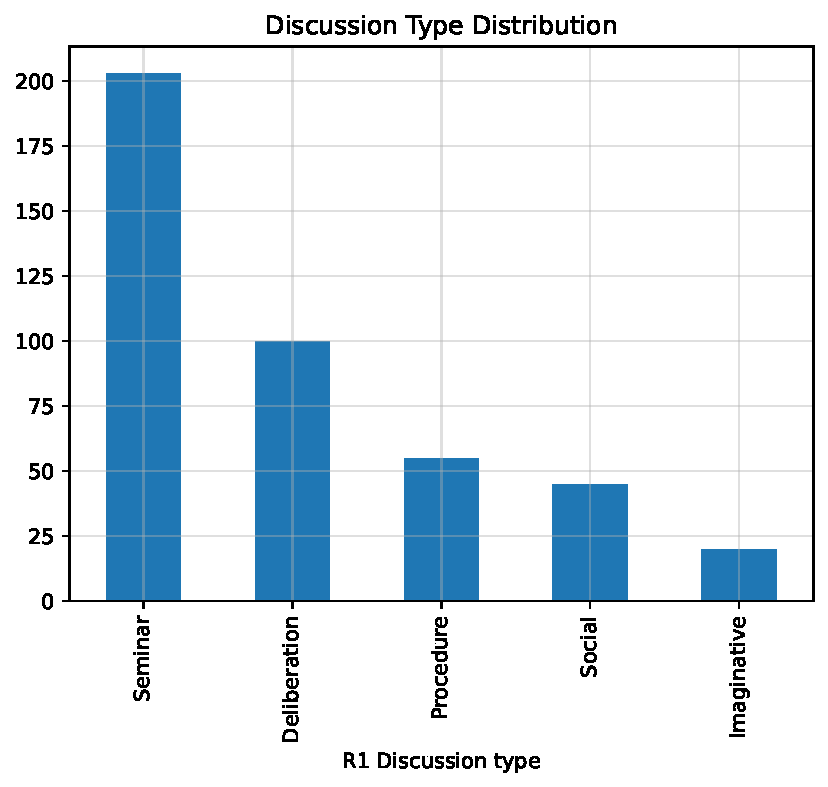
\includegraphics[scale=0.5]{fig/discussion_type_distribution.pdf}
	\caption{Distribution of different discussion types. We can see that 'Seminar' is the predominant type, which is expected from the definition and the type of discourse. The least common type is "Imaginative" which "places the learner in the discussion as an active participant".  }
	\label{fig:distr}
\end{figure}


\iffalse
// UNCOMMENT IF NEEDED //
Additionally, we can analyze the \textit{Pivot} column, which denotes messages that altered the course of discussion, with the formal definition being \textit{The posting establishes or changes the procedural direction of the discussion}. This is evident in Figure \ref{fig:pivot_graph}, where the \textit{Seminar} node occupies the central position with the highest number of connections, aligning with the prevalence of Seminar-type discussions. Outgoing connections are depicted with green arrows, indicating that most pivots originate from \textit{Seminar} and transition into \textit{Deliberation} discussions, and vice versa. This pattern aligns with the definition of \textit{Deliberation} as \textit{Turns related to decision-making about the content}, which often follows or precedes discussions about the story in the \textit{Seminar} type.
 
\begin{figure}[ht!]\centering
	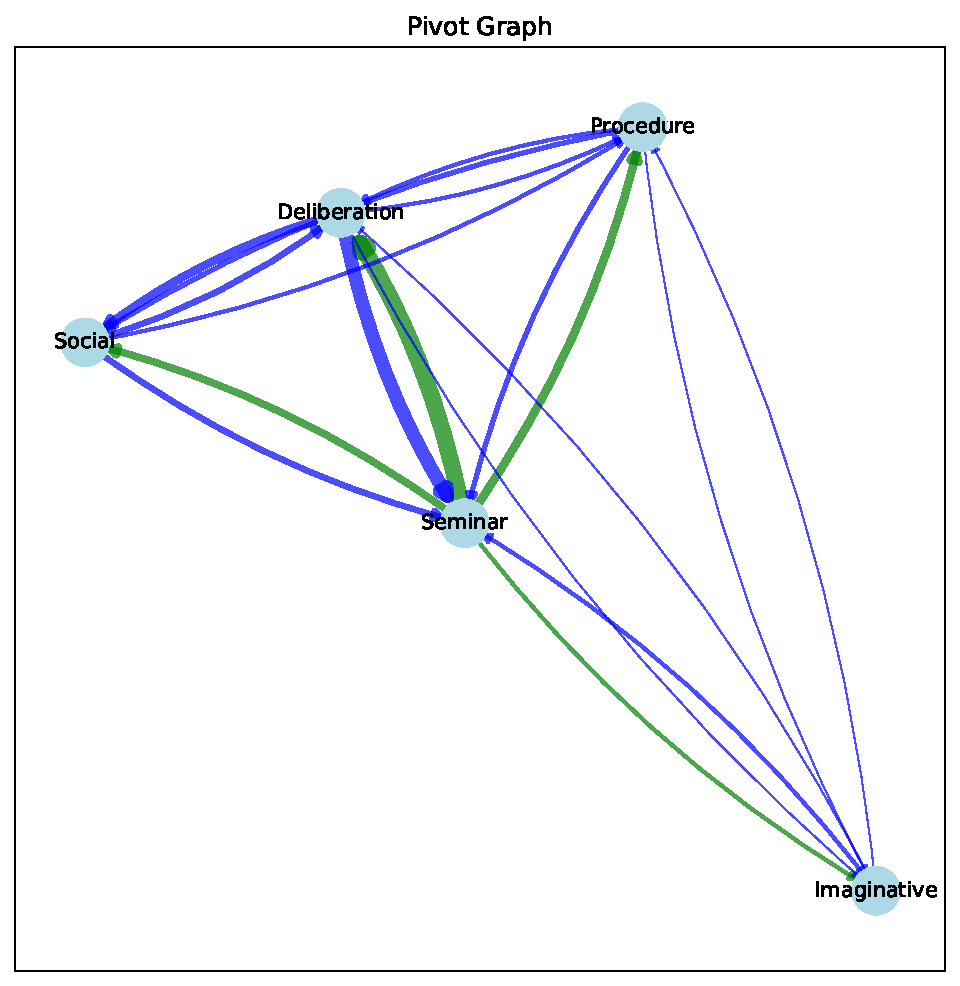
\includegraphics[scale=0.3]{fig/pivot_graph.pdf}
	\caption{The graphical representation illustrates various pivot transitions, with nodes representing different discussion types and lines indicating transitions between them. The width of the lines corresponds to the frequency of specific transitions, while the direction indicates the sequence of occurrences. Notably, thick lines between \textit{Deliberation} and \textit{Seminar} highlight frequent transitions between these two discussion types.}
	\label{fig:pivot_graph}
\end{figure}
\fi


%------------------------------------------------

\section*{Methods}

The main focus of our project is addressing the classification challenge. We chose the \textit{R2DiscussionType} column as our target column as it consistently defines the decision task and serves as the primary class for classification by test subjects. As a benchmark, we employed a pre-trained BERT model (\textit{bert-base-cased}) to classify Discussion types within our dataset. Implementation was carried out using the PyTorch library in Python, which gave us access to Trainer API that we used to fine-tune the pre-trained BERT model. Baseline BERT model was trained with 3 epochs, utilizing a batch size of 8, and employing the standard learning rate of $2 \times 10^{-5}$.

We divided our dataset into three parts: train, test and validation. In the training dataset we have 427 samples or $70\%$ of the dataset, and the test and validation datasets both have 92 samples or $15\%$ of the dataset each. Due to the class imbalance in our dataset, certain less represented classes have only a few samples in the divided datasets. The test dataset is used as an evaluation dataset during the training phase, and we use the validation dataset as a final score of the model.

Using the Trainer API, we also fine-tuned the BERT model by increasing number of epochs. To setup optimizers, we used Adam optimizer by PyTorch and tested a scheduler with implemented \textit{ReduceLROnPlateau}, to reduce learning rate when a metric stops improving.

We also tried using DistilBERT\cite{sanh2020distilbert}, which is a lightweight BERT model fine-tuned for text classification.

We also evaluated several traditional AI models: Multinomial Naive Bayes, Random Forest Classifier, Support Vector Machine (SVM) and XGBoost. We used TF-IDF as the embedding technique to transform the input.   

%% Prompting
In our exploration of advanced NLP techniques for text categorization, we implemented various methodologies centered around the LLAMA2 model \cite{touvron2023llama} and prompt engineering, aiming to enhance the model's ability to perform zero-shot and few-shot prompting. We decided to use LLAMA2, because of it's ability to process 4096 tokens. The LLAMA2 model is highly effective for prompting and text categorization due to several key features. Its fine-tuning with reinforcement learning from human feedback (RLHF) ensures it generates relevant responses based on context. Optimized for dialogue, it handles conversational inputs well, producing coherent replies. With 13 billion parameters, it has a substantial capacity to understand and categorize diverse text accurately. Additionally, its training on a vast dataset of 2 trillion tokens enhances its generalization across topics. Evaluations confirm its performance in terms of safety and helpfulness, making it a reliable choice for various applications.

We chose to perform zero-shot prompting to demonstrate how highly specific text categorization can be achieved using only basic context provided to the LLAMA2 model. In our case, this context consists of category descriptions (Table \ref{tab:category descriptions}) derived from a thorough review of the dataset. This approach offers valuable insights into the model's capability to categorize text accurately without extensive pre-training on the specific task.


To select relevant prompts for few-shot prompting, we reviewed the dataset to extract a representative sample of prompts for each category. We ensured the sample proportions matched the actual distribution of categories in the dataset. This approach tests the model's ability to categorize text using examples from the dataset. Additionally, we enhanced few-shot prompting by providing both examples and descriptions of the categories, aiming to improve the model's categorization performance.

%------------------------------------------------

\section*{Results}
For evaluating our BERT models, we will use micro-F1, or average accuracy, as an evaluation metric to determine how well the model is performing. 

\begin{table}[h!]
\caption{Results of different BERT models with varying epoch number and batch size. We can see that in general bert-large-uncased performs slightly better than others with highest test and validation accuracy. }
\begin{adjustbox}{width=\columnwidth,center}
\begin{tabular}{lllll}
Model               & Epochs & Batch size & Test accuracy & Validation accuracy \\
bert-base-cased     & 3      & 4          & 0.728         & 0.652               \\
bert-base-cased     & 3      & 8          & 0.75          & 0.685               \\
bert-base-cased     & 10     & 8          & 0.77          & 0.696               \\
distil-base-uncased & 10     & 8          & 0.728         & 0.641               \\
distil-base-uncased & 50     & 16         & 0.77          & 0.641             \\
bert-large-uncased & 10     & 8         & 0.72     
& 0.72 \\
bert-large-uncased & 20     & 16         & 0.75        
& 0.72
\end{tabular}
\label{tab:results}
\end{adjustbox}
\end{table}


The best performing model is the large BERT model (\textit{bert-large-uncased}), which has the best accuracy score on the validation dataset. The accuracy is greatly affected by the batch size and the number of epochs in which the model was trained.

\begin{table}[h!]
\caption{Results of traditional AI approaches}
\begin{adjustbox}{width=\columnwidth,center}
\begin{tabular}{lll}
Model & Test accuracy & Validation accuracy \\
Multinomial Naive Bayes & 0.739 & 0.707 \\
Random Forest Classifier & 0.685 & 0.641 \\
Support Vector Machine & 0.739 & 0.641 \\
XGBoost & 0.641 & 0.641 
\end{tabular}
\label{tab:results_trad_AI}
\end{adjustbox}
\end{table}

From the traditional AI models we evaluated, Multinomial Naive Bayes performed best on both the test and validation datasets. Similarly, SVM achieved very good results on the test dataset, but the performance dropped sharply on the validation dataset. 

\begin{table}[h!]
\caption{Results of prompting}
\begin{adjustbox}{width=\columnwidth,center}
\begin{tabular}{lll}
Approach & Test accuracy & Validation accuracy \\
Zero-shot & 0.467 & 0.391 \\
Few-shot & 0.130 & 0.152 \\
Few-shot without category descriptions & 0.152 & 0.174 \\
\end{tabular}
\label{tab:results_prompt}
\end{adjustbox}
\end{table}

In Table \ref{tab:results_prompt} we can see that the best performing prompting approach is zero-shot prompting, while few-shot prompting performs the worst among the models tested in this paper.

%------------------------------------------------

\section*{Discussion}

We can analyze robustness, accuracy, and performance of a specific model through an in-depth examination of instances where the model fails. 

For analysis of the BERT model approach, we used the \textit{bert-base-cased} model, as presented in Table \ref{tab:results}, due to its relatively high accuracy and smaller size. We focused on the incorrect predictions made on the test and validation datasets, which together represent 30\% of the total data. There were a total of 50 erroneous predictions in this subset. The text length of these misclassified instances is visualized in Figure \ref{fig:wrong_pred_len}. Notably, 9 errors occurred in examples where the content length was 20 characters or less. Short examples are considerably harder for BERT to classify correctly due to the limited context available for accurate interpretation. 

In Table \ref{tab:classification_examples}, we present several examples with their corresponding true and predicted labels. Upon inspection, it becomes evident that many of these examples pose significant challenges for classification, indicating the need for additional contextual information to make accurate predictions.

To see which discussion types are more prone to errors, we can analyse a confusion matrix of errors presented in Figure \ref{fig:confusion_matr}. Matrix shows a high amount of examples wrongly predicted as seminar, which may be explained due to large proportion of examples being that type. We can also see a high amount of \textit{UX} examples being classed as \textit{Deliberation}. These errors are often due to the deliberate manner of speech, even though the focus was on UX.

% error analysis for traditional AI approaches
As for the most common misclassification when it comes to the traditional AI models we evaluated, they all most commonly mistook an example which should have been classified as \textit{Deliberation} for \textit{Seminar}. A common pattern was misclassifying examples as \textit{Seminar} or \textit{Deliberation}. Random Forest Classifier, SVM and XGBoost all had similar distributions of wrongly classified examples, whereas Multinomial Naive Bayes mixed up \textit{Procedure} and \textit{Deliberation}, as well as \textit{UX} with \textit{Social}.

% error analysis for prompting
Zero-shot prompting performed well on the test set compared to other prompting approaches, due to a relatively good description of the task and category descriptions. However, it shows a larger difference between accuracy on the test and validation sets compared to other models, although all models underperform on the validation set. This can suggest that the performance is dependent on the testing examples. 
There are numerous instances where LLAMA2 fails to return a category, particularly on the test set. This indicates that LLAMA2 couldn't determine a category based on the given descriptions, as it responded with a plain dash. This suggests that the model struggled with certain inputs (predominantely \textit{Seminar}) and was unable to categorize them effectively using the provided information.


The misclassifications observed in the LLAMA2 zero-shot prompting task can be attributed to several key factors. Primarily, the overlap in category definitions creates significant challenges, as categories such as "Seminar" and "Social" exhibit overlapping characteristics, leading to frequent misclassifications (Figure \ref{fig:zero_shot_combined_cm}). Furthermore, the presence of ambiguous language within the posts exacerbates classification difficulties, as contextually similar language can be interpreted in multiple ways by the model. Some of ambiguous examples are shown in Table \ref{table:misclassifications_prompt}. Additionally, the model’s tendency to generalize based on frequent patterns encountered during training contributes to misclassification, often defaulting to common categories like "Social" when uncertain. The low precision and recall observed for certain categories indicate that the model struggles to accurately identify and differentiate these categories.



Few-shot prompting has shown limited effectiveness in classifying text into the correct categories. This might be due to our prompts not being distinct enough for LLAMA2 to differentiate between categories. Additionally, even when we included category descriptions and examples, the accuracy did not improve significantly. This suggests that the examples may have introduced noise, making the categories less distinguishable. However, in the case of few-shot prompting, LLAMA2 always returns one of the categories, whereas in the case of zero-shot prompting, it sometimes returns none of the categories.

%------------------------------------------------

\section*{Conclusion}
% lahko dodamo v conclusion
% Addressing these challenges requires enhanced prompt design with explicit instructions and refined category definitions. Moreover, fine-tuning the model with a domain-specific labeled dataset would enable it to better learn the nuances of each category, thereby reducing misclassification rates.


In this project, we evaluated several text categorization methods, with our primary focus being qualitative discourse analysis. Our dataset was particularly grounded in reality, as it was comprised of forum posts discussing the story "The Lady, or the Tiger?". 

Due to the nature of the dataset and the overall lack of clear boundaries between the target categories, the models we evaluated struggled with achieving high results. It's noteworthy to mention however, that even traditional machine learning models like Multinomial Naive Bayes and SVM achieved results comparable to our best performing BERT model. While the experiments we did with prompt engineering and LLMs did not achieve the best results, we find there is a lot of potential and future work to be done in this direction. It was with LLAMA where we had the most interesting "errors", whereas the other models had quite similar misclassification distributions. 

Addressing these challenges requires enhanced prompt design with explicit instructions and refined category definitions. Moreover, fine-tuning the model with a domain-specific labeled dataset would enable it to better learn the nuances of each category, thereby reducing misclassification rates. Improving model sensitivity to subtle linguistic cues and reducing misclassification by enhancing training datasets could also help address these issues.

In conclusion, our exploration into the automated categorization of text in online discussions not only advances our understanding of discourse analysis using NLP but also sets the stage for future work to refine these techniques. As AI continues to evolve, its integration into social science research promises to enhance the efficiency and accuracy of qualitative analyses, thereby enriching our understanding of human interaction in digital contexts.

%----------------------------------------------------------------------------------------
%	REFERENCE LIST
%----------------------------------------------------------------------------------------
\bibliographystyle{unsrt}
\bibliography{report}

\appendix
\section*{Appendix}

\begin{figure}[ht!]\centering
	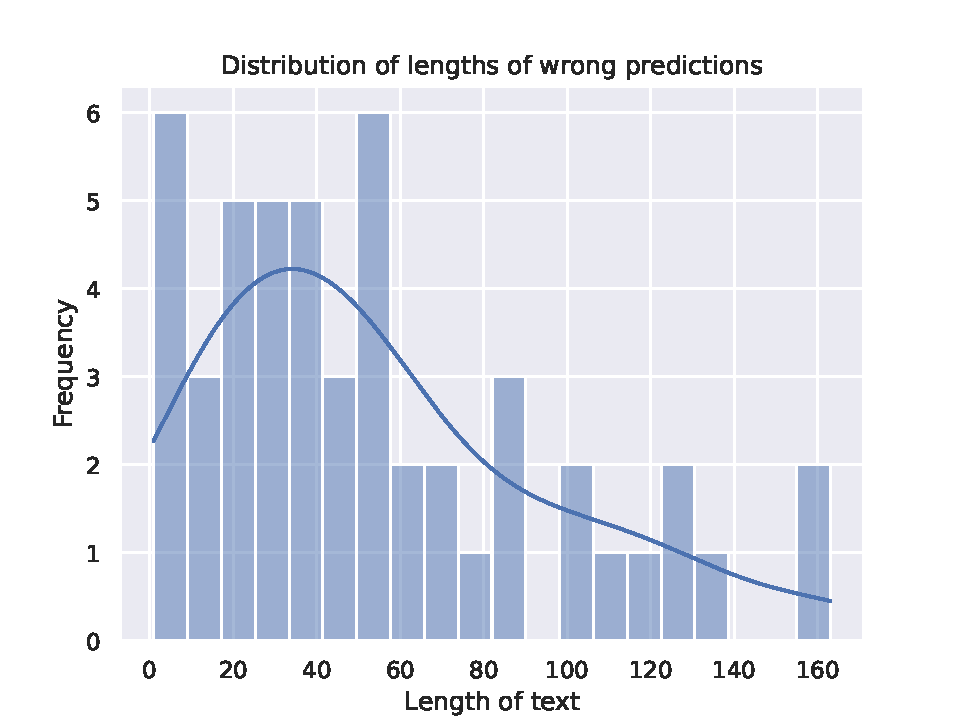
\includegraphics[scale=0.5]{fig/wrong_predictions_length_distribution.pdf}
	\caption{Histogram showing the distribution of the lengths of incorrectly predicted text. Numerous examples have a length of less than 20 characters, posing a challenge for BERT.}
	\label{fig:wrong_pred_len}
\end{figure}


\begin{figure}[]\centering
	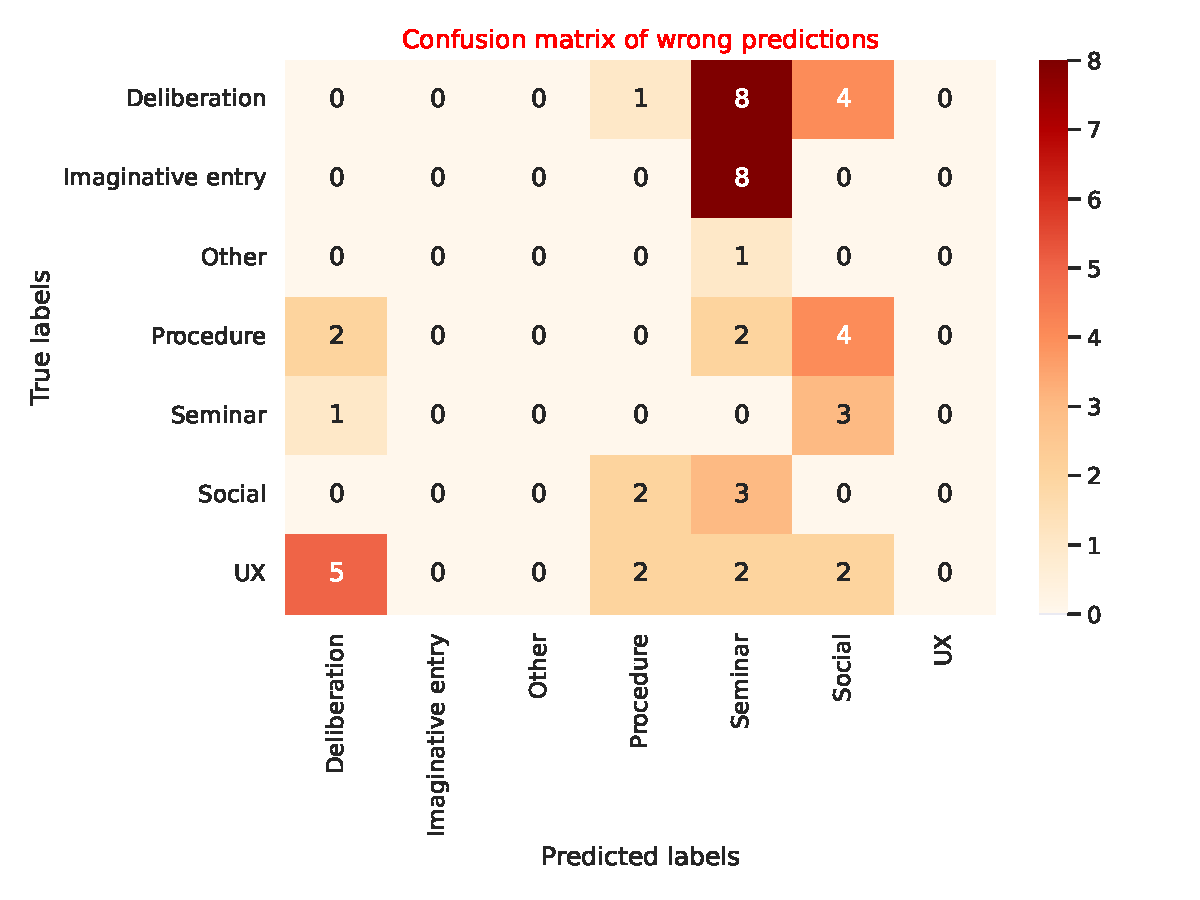
\includegraphics[scale=0.4]{fig/confusion_matrix_wrong_predictions.pdf}
	\caption{Confusion matrix representing true labels on horizontal and predicted labels on vertical lines. Unsurprisingly, many text cases are classified as seminar, due to its predominance in the dataset. }
	\label{fig:confusion_matr}
\end{figure}


\begin{figure}[ht!]\centering
	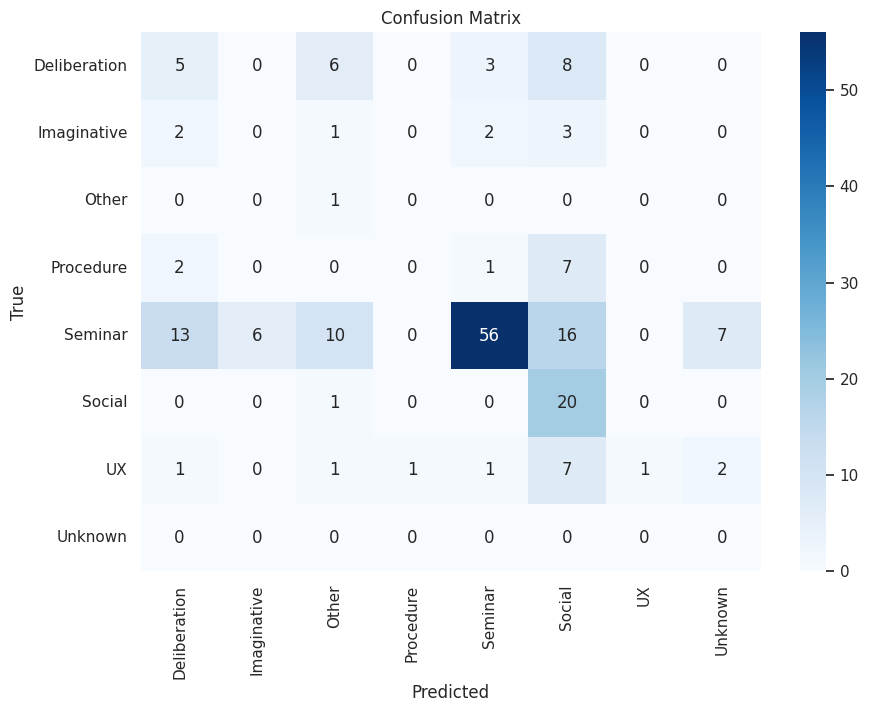
\includegraphics[scale=0.4]{fig/zero-shot-combined_cm_2.png}
	\caption{Confusion matrix of classification by zero-shot prompting on combined set of test and validation set.
Many text of category \textit{Seminar} cases are classified as \textit{Social} and \textit{Deliberation}, due to overlap in category definitions.}
	\label{fig:zero_shot_combined_cm}
\end{figure}


\begin{table}[h!]
\caption{Descriptions of each category}
\begin{adjustbox}{width=\columnwidth,center}
\begin{tabular}{l|p{8cm}}
Category & Description\\
\hline
Seminar & \textit{Posts discussing the deeper meanings of content, encouraging analysis and interpretation.} \\
Deliberation & \textit{Posts about making decisions, often involving questions and considerations for future actions.}\\
Social & \textit{Posts to establish or maintain relationships, often casual and friendly in nature.} \\
UX & \textit{Posts discussing the user experience, including issues and feedback about interfaces and usability.} \\
Procedure & \textit{Posts about accomplishing a task, often with step-by-step instructions or suggestions for organizing activities.} \\
Imaginative & \textit{Posts about imaginative content, often involving hypothetical scenarios or creative storytelling.}\\
Other & \textit{Posts that do not fit into any of the above categories.}\\
\end{tabular}
\label{tab:category descriptions}
\end{adjustbox}
\end{table}

\begin{table}[ht!]
\caption{Examples of short text misclassifications with true and predicted labels.}
\begin{adjustbox}{width=\columnwidth,center}
\centering
\begin{tabular}{|p{5cm}|p{3cm}|p{3cm}|}
\hline
\textbf{Text} & \textbf{True Label} & \textbf{Predicted Label} \\
\hline
I like it & Deliberation & Seminar \\
Submitted & Deliberation & Social \\
w & Other & Seminar \\
And that's true! & Imaginative entry & Seminar \\
Good idea. & Seminar & Social \\
I am on, & Procedure & Deliberation \\
I couldn't either. & Procedure & Seminar \\
it's wonderful! & Seminar & Social \\
ok & Deliberation & Social \\
ooooh & UX & Social \\
\hline
\end{tabular}
\label{tab:classification_examples}
\end{adjustbox}
\end{table} 

\begin{table}[ht!]
\caption{Examples of short text misclassifications with true and predicted labels with prompting.}
\begin{adjustbox}{width=\columnwidth,center}
\centering
\begin{tabular}{|p{5cm}|c|c|}
\hline
\textbf{Text} & \textbf{True Label} & \textbf{Predicted Label} \\
\hline
Did you guys already read the story? It won't move past the part of four questions for me. & UX & Social \\
And that's true! & Imaginative & Social \\ 
Oh that would be a good punishment for her! & Seminar & Social \\ 
Would the king even entertain that idea given it is his daughter? & Seminar & Deliberation \\ 
What would happen then? & Seminar & Imaginative \\ 
I'm not sure. They're probably equally beautiful and just jealous :) & Seminar & Social \\ \hline
\end{tabular}
\label{table:misclassifications_prompt}
\end{adjustbox}
\end{table} 

\end{document}